

\tikzset{every picture/.style={line width=0.75pt}} %set default line width to 0.75pt        

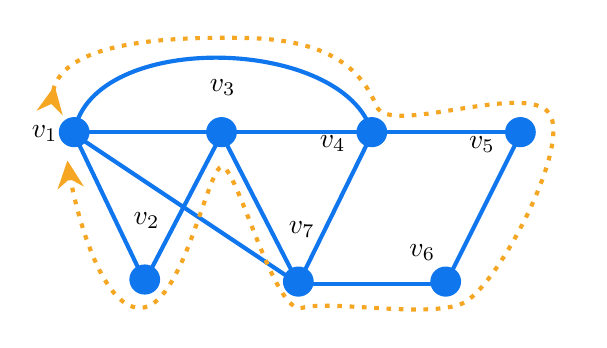
\begin{tikzpicture}[x=0.75pt,y=0.75pt,yscale=-1,xscale=1]
%uncomment if require: \path (0,163); %set diagram left start at 0, and has height of 163

%Curve Lines [id:da7683292464406222] 
\draw [color={rgb, 255:red, 15; green, 118; blue, 237 }  ,draw opacity=1 ][line width=1.5]    (36.33,57.67) .. controls (45.1,8.34) and (166.1,11.34) .. (179.74,57.67) ;
%Straight Lines [id:da08884414649664008] 
\draw [color={rgb, 255:red, 15; green, 118; blue, 237 }  ,draw opacity=1 ][line width=1.5]    (36.33,58.67) -- (70.33,129.67) ;
%Straight Lines [id:da48325776435904766] 
\draw [color={rgb, 255:red, 15; green, 118; blue, 237 }  ,draw opacity=1 ][line width=1.5]    (70.33,129.67) -- (107.33,58.67) ;
%Straight Lines [id:da5108779557079501] 
\draw [color={rgb, 255:red, 15; green, 118; blue, 237 }  ,draw opacity=1 ][line width=1.5]    (144.33,130.67) -- (107.33,58.67) ;
%Straight Lines [id:da42357082617222597] 
\draw [color={rgb, 255:red, 15; green, 118; blue, 237 }  ,draw opacity=1 ][line width=1.5]    (144.33,130.67) -- (215.33,130.67) ;
%Straight Lines [id:da07152389857292141] 
\draw [color={rgb, 255:red, 15; green, 118; blue, 237 }  ,draw opacity=1 ][line width=1.5]    (215.33,130.67) -- (251.33,58.67) ;
%Straight Lines [id:da7119953651174364] 
\draw [color={rgb, 255:red, 15; green, 118; blue, 237 }  ,draw opacity=1 ][line width=1.5]    (179.74,57.67) -- (251.33,57.67) ;
%Shape: Ellipse [id:dp5075093592027435] 
\draw  [draw opacity=0][fill={rgb, 255:red, 15; green, 118; blue, 237 }  ,fill opacity=1 ] (28.92,57.67) .. controls (28.92,53.66) and (32.24,50.41) .. (36.33,50.41) .. controls (40.42,50.41) and (43.74,53.66) .. (43.74,57.67) .. controls (43.74,61.69) and (40.42,64.94) .. (36.33,64.94) .. controls (32.24,64.94) and (28.92,61.69) .. (28.92,57.67) -- cycle ;
%Shape: Ellipse [id:dp13603931445795947] 
\draw  [draw opacity=0][fill={rgb, 255:red, 15; green, 118; blue, 237 }  ,fill opacity=1 ] (99.92,57.67) .. controls (99.92,53.66) and (103.24,50.41) .. (107.33,50.41) .. controls (111.42,50.41) and (114.74,53.66) .. (114.74,57.67) .. controls (114.74,61.69) and (111.42,64.94) .. (107.33,64.94) .. controls (103.24,64.94) and (99.92,61.69) .. (99.92,57.67) -- cycle ;
%Shape: Ellipse [id:dp7516959175994735] 
\draw  [draw opacity=0][fill={rgb, 255:red, 15; green, 118; blue, 237 }  ,fill opacity=1 ] (172.33,57.67) .. controls (172.33,53.66) and (175.65,50.41) .. (179.74,50.41) .. controls (183.83,50.41) and (187.15,53.66) .. (187.15,57.67) .. controls (187.15,61.69) and (183.83,64.94) .. (179.74,64.94) .. controls (175.65,64.94) and (172.33,61.69) .. (172.33,57.67) -- cycle ;
%Shape: Ellipse [id:dp9678063492720343] 
\draw  [draw opacity=0][fill={rgb, 255:red, 15; green, 118; blue, 237 }  ,fill opacity=1 ] (243.92,57.67) .. controls (243.92,53.66) and (247.24,50.41) .. (251.33,50.41) .. controls (255.42,50.41) and (258.74,53.66) .. (258.74,57.67) .. controls (258.74,61.69) and (255.42,64.94) .. (251.33,64.94) .. controls (247.24,64.94) and (243.92,61.69) .. (243.92,57.67) -- cycle ;
%Shape: Ellipse [id:dp9669459656751889] 
\draw  [draw opacity=0][fill={rgb, 255:red, 15; green, 118; blue, 237 }  ,fill opacity=1 ] (62.92,128.67) .. controls (62.92,124.66) and (66.24,121.41) .. (70.33,121.41) .. controls (74.42,121.41) and (77.74,124.66) .. (77.74,128.67) .. controls (77.74,132.69) and (74.42,135.94) .. (70.33,135.94) .. controls (66.24,135.94) and (62.92,132.69) .. (62.92,128.67) -- cycle ;
%Shape: Ellipse [id:dp9141299370953122] 
\draw  [draw opacity=0][fill={rgb, 255:red, 15; green, 118; blue, 237 }  ,fill opacity=1 ] (136.92,129.67) .. controls (136.92,125.66) and (140.24,122.41) .. (144.33,122.41) .. controls (148.42,122.41) and (151.74,125.66) .. (151.74,129.67) .. controls (151.74,133.69) and (148.42,136.94) .. (144.33,136.94) .. controls (140.24,136.94) and (136.92,133.69) .. (136.92,129.67) -- cycle ;
%Shape: Ellipse [id:dp5433101163289387] 
\draw  [draw opacity=0][fill={rgb, 255:red, 15; green, 118; blue, 237 }  ,fill opacity=1 ] (207.92,129.67) .. controls (207.92,125.66) and (211.24,122.41) .. (215.33,122.41) .. controls (219.42,122.41) and (222.74,125.66) .. (222.74,129.67) .. controls (222.74,133.69) and (219.42,136.94) .. (215.33,136.94) .. controls (211.24,136.94) and (207.92,133.69) .. (207.92,129.67) -- cycle ;
%Straight Lines [id:da21140953542973562] 
\draw [color={rgb, 255:red, 15; green, 118; blue, 237 }  ,draw opacity=1 ][line width=1.5]    (36.33,58.67) -- (144.33,130.67) ;
%Straight Lines [id:da4547447000051603] 
\draw [color={rgb, 255:red, 15; green, 118; blue, 237 }  ,draw opacity=1 ][line width=1.5]    (36.33,57.67) -- (107.33,57.67) ;
%Straight Lines [id:da9169893513605827] 
\draw [color={rgb, 255:red, 15; green, 118; blue, 237 }  ,draw opacity=1 ][line width=1.5]    (107.33,57.67) -- (179.74,57.67) ;
%Straight Lines [id:da8670329719288252] 
\draw [color={rgb, 255:red, 15; green, 118; blue, 237 }  ,draw opacity=1 ][line width=1.5]    (144.33,130.67) -- (179.74,58.67) ;
%Curve Lines [id:da030458729127779582] 
\draw [color={rgb, 255:red, 245; green, 166; blue, 35 }  ,draw opacity=1 ][line width=1.5]  [dash pattern={on 1.69pt off 2.76pt}]  (26.26,37.55) .. controls (31.35,15.22) and (76.61,11.35) .. (120.1,12.34) .. controls (164.1,13.34) and (176.1,31.34) .. (182.1,45.34) .. controls (188.1,59.34) and (249.88,34.55) .. (264.1,47.34) .. controls (278.33,60.13) and (240.1,133.34) .. (223.1,140.34) .. controls (206.1,147.34) and (159.61,138.4) .. (146.1,142.34) .. controls (132.6,146.28) and (114.1,71.34) .. (107.1,74.34) .. controls (100.1,77.34) and (88.42,142.28) .. (68.1,142.34) .. controls (49.11,142.4) and (36.78,95.14) .. (33.63,75.1) ;
\draw [shift={(33.1,71.34)}, rotate = 443.29] [fill={rgb, 255:red, 245; green, 166; blue, 35 }  ,fill opacity=1 ][line width=0.08]  [draw opacity=0] (13.4,-6.43) -- (0,0) -- (13.4,6.44) -- (8.9,0) -- cycle    ;
\draw [shift={(26.92,35.34)}, rotate = 460.31] [fill={rgb, 255:red, 245; green, 166; blue, 35 }  ,fill opacity=1 ][line width=0.08]  [draw opacity=0] (13.4,-6.43) -- (0,0) -- (13.4,6.44) -- (8.9,0) -- cycle    ;

% Text Node
\draw (14.43,52.78) node [anchor=north west][inner sep=0.75pt]    {$v_{1}$};
% Text Node
\draw (63.5,95.05) node [anchor=north west][inner sep=0.75pt]    {$v_{2}$};
% Text Node
\draw (100.18,30.8) node [anchor=north west][inner sep=0.75pt]    {$v_{3}$};
% Text Node
\draw (153.16,57.62) node [anchor=north west][inner sep=0.75pt]    {$v_{4}$};
% Text Node
\draw (225.09,58.42) node [anchor=north west][inner sep=0.75pt]    {$v_{5}$};
% Text Node
\draw (196.33,110.15) node [anchor=north west][inner sep=0.75pt]    {$v_{6}$};
% Text Node
\draw (138.33,99.15) node [anchor=north west][inner sep=0.75pt]    {$v_{7}$};


\end{tikzpicture}